\documentclass[12pt,a4paper]{article}

% ─── Page Layout ───────────────────────────────────────────────────────────────
\usepackage[a4paper, margin=0.8in, headheight=14pt]{geometry}

% ─── Fonts (XeLaTeX) ───────────────────────────────────────────────────────────
\usepackage{fontspec}
\usepackage{unicode-math}
\setmainfont{TeX Gyre Pagella}
\setmonofont[Scale=0.88]{TeX Gyre Cursor}
\setmathfont{Latin Modern Math}

% ─── Packages ──────────────────────────────────────────────────────────────────
\usepackage{xcolor}
\usepackage{colortbl}
\usepackage{titlesec}
\usepackage{enumitem}
\usepackage{tabularx}
\usepackage{booktabs}
\usepackage{array}
\usepackage{amsmath}
\usepackage{tikz}
\usetikzlibrary{shapes.geometric, arrows.meta, positioning, calc, fit, decorations.pathreplacing, patterns}
\usepackage{tcolorbox}
\tcbuselibrary{skins, breakable}
\usepackage{hyperref}
\usepackage{fancyhdr}
\usepackage{graphicx}
\usepackage{microtype}
\hyphenpenalty=10000
\exhyphenpenalty=10000
\sloppy
\usepackage{caption}
\usepackage{setspace}
\usepackage{multirow}
\usepackage{tocloft}

% ─── Q&A helper ────────────────────────────────────────────────────────────────
\newcommand{\Q}[1]{\textbf{#1}\par\noindent\ignorespaces}

% ─── Colour Palette ────────────────────────────────────────────────────────────
\definecolor{myred}{RGB}{196,30,58}
\definecolor{mydark}{RGB}{30,30,50}
\definecolor{mygreen}{RGB}{14,120,80}
\definecolor{myteal}{RGB}{0,130,140}
\definecolor{myamber}{RGB}{180,100,0}
\definecolor{mypurple}{RGB}{100,30,160}
\definecolor{mygray}{RGB}{246,247,249}
\definecolor{mgframe}{RGB}{180,185,200}
\definecolor{watermark}{RGB}{145,150,170}
\definecolor{hdrred}{RGB}{250,232,235}
\definecolor{hdrgreen}{RGB}{220,244,233}
\definecolor{hdrteal}{RGB}{220,242,244}
\definecolor{hdramber}{RGB}{253,242,215}
\definecolor{hdrpurple}{RGB}{238,228,255}
\definecolor{hdrgray}{RGB}{238,240,245}
\definecolor{rowalt}{RGB}{250,251,253}

% ─── Section Formatting ────────────────────────────────────────────────────────
\titleformat{\section}{\large\bfseries\color{myred}}{\thesection.}{0.5em}{}[\vspace{1pt}{\color{myred}\rule{\linewidth}{0.8pt}}]
\titleformat{\subsection}{\normalsize\bfseries\color{myteal}}{\thesubsection}{0.5em}{}
\titlespacing*{\section}{0pt}{18pt}{7pt}
\titlespacing*{\subsection}{0pt}{11pt}{4pt}

% ─── Paragraph ─────────────────────────────────────────────────────────────────
\setlength{\parindent}{0pt}
\setlength{\parskip}{4pt}

% ─── TOC Styling ───────────────────────────────────────────────────────────────
\renewcommand{\cfttoctitlefont}{\large\bfseries\color{myred}}
\renewcommand{\cftaftertoctitle}{\par\noindent{\color{myred}\rule{\linewidth}{0.8pt}}}
\setlength{\cftbeforetoctitleskip}{0pt}
\setlength{\cftaftertoctitleskip}{6pt}
\renewcommand{\cftsecfont}{\normalsize\bfseries\color{mydark}}
\renewcommand{\cftsecpagefont}{\normalsize\bfseries\color{mydark}}
\renewcommand{\cftsecleader}{\cftdotfill{\cftdotsep}}
\setlength{\cftbeforesecskip}{7pt}
\renewcommand{\cftsubsecfont}{\small\color{mydark}}
\renewcommand{\cftsubsecpagefont}{\small\color{mydark}}
\setlength{\cftbeforesubsecskip}{3pt}
\setlength{\cftsubsecindent}{1.4em}

% ─── Table helpers ─────────────────────────────────────────────────────────────
\renewcommand{\arraystretch}{1.45}
\setlength{\tabcolsep}{6pt}
\arrayrulecolor{mydark}
\newcolumntype{B}[1]{>{\small\bfseries\raggedright\arraybackslash}m{#1}}
\newcolumntype{Y}{>{\small\raggedright\arraybackslash}X}
\renewcommand{\tabularxcolumn}[1]{m{#1}}

% ─── Header / Footer ───────────────────────────────────────────────────────────
\pagestyle{fancy}
\fancyhf{}
\fancyhead[L]{\small\color{myred}\textbf{OE-EC803A}\;\color{mydark}--- Internet of Things}
\fancyhead[R]{\small\color{myteal}\textbf{Module 1 Notes}}
\fancyfoot[C]{\small\color{mydark}\thepage}
\fancyfoot[R]{\small\color{watermark}\textit{\copyright\ Biraj Sarkar}}
\renewcommand{\headrulewidth}{0.5pt}
\renewcommand{\footrulewidth}{0.3pt}

% ─── Hyperref ──────────────────────────────────────────────────────────────────
\hypersetup{colorlinks=true, linkcolor=myteal, urlcolor=myteal,
  pdfauthor={Biraj Sarkar}, pdftitle={OE-EC803A --- Module 1 Notes}}

% ─── tcolorbox styles ──────────────────────────────────────────────────────────
\tcbset{
  tikzbox/.style={colback=mygray, colframe=mgframe, boxrule=0.6pt, arc=4pt,
    left=8pt, right=8pt, top=6pt, bottom=6pt,
    colbacktitle=mgframe, coltitle=mydark, fonttitle=\small\bfseries},
  defbox/.style={colback=hdrgreen, colframe=mygreen, boxrule=0.8pt, arc=4pt,
    left=9pt, right=9pt, top=6pt, bottom=6pt,
    colbacktitle=mygreen, coltitle=white, fonttitle=\small\bfseries},
  formulabox/.style={colback=hdrteal, colframe=myteal, boxrule=0.8pt, arc=4pt,
    left=9pt, right=9pt, top=7pt, bottom=7pt,
    colbacktitle=myteal, coltitle=white, fonttitle=\small\bfseries},
  examplebox/.style={colback=hdramber, colframe=myamber, boxrule=0.8pt, arc=4pt,
    left=9pt, right=9pt, top=6pt, bottom=6pt,
    colbacktitle=myamber, coltitle=white, fonttitle=\small\bfseries},
  masonbox/.style={colback=hdrpurple, colframe=mypurple, boxrule=0.8pt, arc=4pt,
    left=9pt, right=9pt, top=6pt, bottom=6pt,
    colbacktitle=mypurple, coltitle=white, fonttitle=\small\bfseries},
  exambox/.style={colback=hdrpurple, colframe=mypurple, boxrule=1pt, arc=5pt,
    left=10pt, right=10pt, top=8pt, bottom=8pt,
    colbacktitle=mypurple, coltitle=white, fonttitle=\bfseries,
    breakable, title after break={\textbf{Frequently Asked / Viva Questions (contd.)}}}
}
\tcbset{breakable}

% ─── TikZ styles ───────────────────────────────────────────────────────────────
\tikzset{
  block/.style={rectangle, draw=myteal, fill=hdrteal,
    text width=2.5cm, align=center, minimum height=1.0cm,
    font=\small, rounded corners=3pt, line width=0.7pt},
  redblock/.style={rectangle, draw=myred, fill=hdrred,
    text width=2.5cm, align=center, minimum height=1.0cm,
    font=\small, rounded corners=3pt, line width=0.7pt},
  arrow/.style={-Stealth, thick, color=mydark},
  line/.style={draw, thick, color=mydark}
}

\begin{document}

% ═══════════════════════════════════════════════════════════════════════════════
% TITLE BLOCK
% ═══════════════════════════════════════════════════════════════════════════════
\begin{center}
  \hfill \textit{Exam-Ready Short Notes} \\
  \vspace{6pt}
  {\LARGE\bfseries\color{myred} OE-EC803A --- Internet of Things}\\[5pt]
  {\normalsize\color{mydark} Semester VIII \quad$\bullet$\quad 3L:0T:0P \quad$\bullet$\quad 3 Credits}\\[3pt]
  {\normalsize\color{myteal}\textbf{Module 1: Introduction to IoT \& Design Principles}}\\[3pt]
  {\small\color{mydark} CGEC \;$|$\; B.Tech ECE (2023--27) \;$|$\; \textit{Biraj Sarkar}}
\end{center}
\vspace{2pt}
\noindent{\color{myred}\rule{\linewidth}{1.5pt}}
\vspace{2pt}

\hypersetup{linkcolor=mydark}
\tableofcontents
\hypersetup{linkcolor=myteal}
\newpage

% ===============================================================================
\section{The Internet of Things: An Overview}
% ===============================================================================

\begin{tcolorbox}[defbox, title={Internet of Things (IoT)}]
  \textbf{The Internet of Things (IoT)} is a global network of physically interconnected objects (or ``things'') embedded with sensors, software, actuators, and network connectivity, enabling them to collect, exchange, and act on data without requiring direct human-to-human or human-to-computer interaction.
\end{tcolorbox}

\subsection{The Flavour of the Internet of Things}
IoT bridges the gap between the physical and digital worlds by introducing \textbf{digital identity} and \textbf{intelligence} to everyday objects.
\begin{itemize}[leftmargin=*, itemsep=3pt]
  \item \textbf{Physical-Digital Convergence:} Traditional devices (like a toaster or street light) are passive. IoT transforms them into active entities that communicate status and receive remote commands.
  \item \textbf{M2M (Machine-to-Machine) vs. IoT:} While M2M refers to point-to-point communication between hardware devices over dedicated lines (often isolated), IoT represents IP-based communication connecting billions of heterogeneous devices globally through standard internet protocols.
\end{itemize}

\par\vspace{6pt}\noindent
{\renewcommand{\arraystretch}{1.35}%
\begin{tabularx}{\linewidth}{|B{3.2cm}|Y|Y|}
\hline
\textbf{Parameter} & \textbf{Traditional Embedded System} & \textbf{Internet of Things (IoT)} \\
\hline
Connectivity & None or local point-to-point (isolated). & IP-based internet connection (global routing). \\
\hline
Data Processing & Local execution on microcontroller. & Distributed processing (Edge + Cloud computing). \\
\hline
Human Interaction & Direct interface (buttons, LCD screen). & Ambient, screenless, or remote app interaction. \\
\hline
Scale & Standalone, singular execution. & Interconnected, heterogeneous device fleets. \\
\hline
\end{tabularx}}

\subsection{The Technology of the Internet of Things}
The IoT system is built upon a multi-tier architectural stack:
\begin{enumerate}[leftmargin=*, itemsep=3pt]
  \item \textbf{Edge Layer (Physical/Perception):} Comprises sensors (LDR, DHT11) to collect parameters and actuators (relays, motors) to execute physical actions.
  \item \textbf{Network/Gateway Layer:} Connects edge nodes to the cloud. Handles protocol translation, packet routing, and local data filtering.
  \item \textbf{Cloud/Application Layer:} Analyzes incoming data streams, executes business logic, manages databases, and provides API endpoints and user dashboards.
\end{enumerate}

\begin{tcolorbox}[tikzbox, title={IoT 3-Tier Architecture Hierarchy}]
\centering
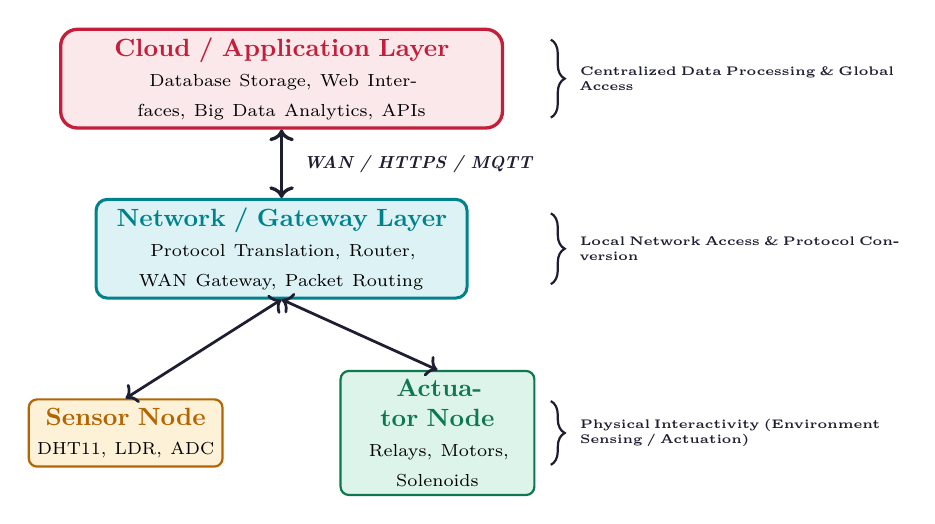
\begin{tikzpicture}[scale=0.9, transform shape]
  % Cloud Layer (Top)
  \node[draw=myred, fill=hdrred, rounded corners=6pt, line width=1.2pt, text width=6.0cm, align=center, minimum height=1.1cm] (cloud) at (0,4.8) {
    \textbf{\color{myred}Cloud / Application Layer}\\
    \scriptsize Database Storage, Web Interfaces, Big Data Analytics, APIs
  };

  % Gateway Layer (Middle)
  \node[draw=myteal, fill=hdrteal, rounded corners=4pt, line width=1.1pt, text width=5.0cm, align=center, minimum height=1.0cm] (gate) at (0,2.4) {
    \textbf{\color{myteal}Network / Gateway Layer}\\
    \scriptsize Protocol Translation, Router, WAN Gateway, Packet Routing
  };

  % Edge Nodes (Bottom)
  \node[draw=myamber, fill=hdramber, rounded corners=3pt, line width=0.8pt, text width=2.5cm, align=center, minimum height=0.9cm] (sensor) at (-2.2,-0.2) {
    \textbf{\color{myamber}Sensor Node}\\
    \scriptsize DHT11, LDR, ADC
  };

  \node[draw=mygreen, fill=hdrgreen, rounded corners=3pt, line width=0.8pt, text width=2.5cm, align=center, minimum height=0.9cm] (actuator) at (2.2,-0.2) {
    \textbf{\color{mygreen}Actuator Node}\\
    \scriptsize Relays, Motors, Solenoids
  };

  % Connections
  \draw[arrow, <->, line width=1.2pt, color=mydark] (cloud) -- node[right=5pt, font=\scriptsize\itshape\bfseries] {WAN / HTTPS / MQTT} (gate);
  \draw[arrow, <->, line width=1.0pt, color=mydark] (gate.south) -- (sensor.north);
  \draw[arrow, <->, line width=1.0pt, color=mydark] (gate.south) -- (actuator.north);

  % Labels/Side brackets - Vertically aligned at X=3.8
  \draw[thick, decoration={brace, amplitude=5pt}, decorate, color=mydark] (3.8, 5.35) -- (3.8, 4.25) 
    node[midway, right=8pt, font=\tiny\bfseries, text width=4.5cm, align=left] {Centralized Data Processing \& Global Access};

  \draw[thick, decoration={brace, amplitude=5pt}, decorate, color=mydark] (3.8, 2.90) -- (3.8, 1.90) 
    node[midway, right=8pt, font=\tiny\bfseries, text width=4.5cm, align=left] {Local Network Access \& Protocol Conversion};

  \draw[thick, decoration={brace, amplitude=5pt}, decorate, color=mydark] (3.8, 0.25) -- (3.8, -0.65) 
    node[midway, right=8pt, font=\tiny\bfseries, text width=4.5cm, align=left] {Physical Interactivity (Environment Sensing / Actuation)};
\end{tikzpicture}
\end{tcolorbox}

\subsection{Enchanted Objects}
The term \textbf{Enchanted Objects}, coined by MIT media lab researcher David Rose, refers to ordinary physical objects that are enhanced with localized, ambient technology to display information or react to user actions without demanding their full cognitive attention.
\begin{itemize}[leftmargin=*, itemsep=2pt]
  \item Instead of forcing users to look at a glowing smartphone screen, information is embedded naturally into the physical environment.
  \item \textbf{Example:} An \textit{Ambient Orb} that glows red if the stock market goes down, or blue if it goes up. The information is consumed at a glance, blending into the background.
\end{itemize}

David Rose classifies these objects according to \textbf{six fundamental human desires}:
\begin{enumerate}[leftmargin=*, itemsep=2.5pt]
  \item \textbf{Omniscience (All-Knowing):} Objects that provide information, such as the \textit{Ambient Umbrella} that glows when it is going to rain.
  \item \textbf{Telepathy (Communication):} Objects that allow remote emotional connection, like \textit{connected lamps} that light up when touched by a loved one.
  \item \textbf{Safekeeping (Protection):} Objects that track security, like smart door locks or GPS-connected wallets.
  \item \textbf{Health and Vitality:} Wearables or pill bottles that track dosage compliance and body vitals.
  \item \textbf{Teleportation (Locomotion):} Devices that bridge spatial distance, such as smart cameras or remote-controlled vehicles.
  \item \textbf{Expression (Creativity):} Instruments and smart surfaces that adapt dynamically to user expressions.
\end{enumerate}

\subsection{Who is Making the Internet of Things?}
The IoT ecosystem is built by a diverse group of creators across three main levels:
\begin{itemize}[leftmargin=*, itemsep=3.0pt]
  \item \textbf{Makers and Hobbyists:} Individuals using open-source hardware (Arduino, Raspberry Pi) and software libraries to build custom DIY projects. They drive rapid community innovation.
  \item \textbf{Startups:} Lean companies developing niche connected products (e.g. smart pet feeders, fitness wearables) and leveraging crowdfunding to prove market demand.
  \item \textbf{Tech Giants and Enterprises:} Large corporations (like Bosch, Cisco, Siemens, Google, Apple, and AWS) that design industrial IoT (IIoT) platforms, establish global protocols, and build massive cloud infrastructure to manage billions of nodes.
\end{itemize}


% ===============================================================================
\section{Design Principles for Connected Devices}
% ===============================================================================

Designing connected products requires moving away from the mouse-and-keyboard paradigm toward natural physical interfaces.

\subsection{Calm and Ambient Technology}
\begin{tcolorbox}[defbox, title={Calm Technology}]
  \textbf{Calm Technology}, formulated by Mark Weiser and John Seely Brown, is hardware/software design that informs the user but remains in the periphery of their attention, moving smoothly between the center and the margin of user focus.
\end{tcolorbox}
\begin{itemize}[leftmargin=*, itemsep=2.5pt]
  \item \textbf{Periphery Concept:} The human brain processes peripheral cues constantly (like the hum of an engine or wind blowing). Calm design uses these peripheral channels to present digital information, minimizing cognitive load.
  \item \textbf{Ambient Displays:} Use light, sound, or physical motion to convey information subtly (e.g., a smart umbrella handle that glows when rain is in the local forecast).
\end{itemize}

Mark Weiser and John Seely Brown characterized the shift in computing history across three main eras:
\begin{itemize}[leftmargin=*, itemsep=2.5pt]
  \item \textbf{Mainframe Era:} One computer shared by many people. High complexity and high cognitive distance.
  \item \textbf{Personal Computer (PC) Era:} One computer per person. Active screen attention, leading to information overload.
  \item \textbf{Ubiquitous/Calm Computing Era:} Many computers per person. Technology recedes into the physical background, operating in our peripheral attention.
\end{itemize}

\subsection{Magic as Metaphor}
When designing connected objects, users often conceptualize digital capabilities as ``magic'' (e.g. a mirror that displays weather, or a key that tracks its location).
\begin{itemize}[leftmargin=*, itemsep=2pt]
  \item Metaphors from fairy tales (such as crystal balls, magic wands, and mirrors) serve as design patterns for natural user interfaces.
  \item The technology should remain invisible; the user interacts directly with the physical object, not the screen/interface.
\end{itemize}

\subsection{Web Thinking for Connected Devices}
Applying Web principles to physical hardware is called the \textbf{Web of Things (WoT)}:
\begin{itemize}[leftmargin=*, itemsep=3pt]
  \item \textbf{Loose Coupling:} Connected devices should be modular and independent. Changing the cloud backend should not brick the physical device.
  \item \textbf{RESTful Architectures:} Representing physical actions as resources using standard HTTP verbs (e.g., `POST /livingroom/light` to turn on a lamp).
  \item \textbf{Open Standards:} Prefer open APIs, JSON, and TCP/IP protocols over proprietary closed stacks to prevent vendor lock-in.
\end{itemize}

\subsection{Affordances}
\begin{tcolorbox}[defbox, title={Affordance}]
  An \textbf{Affordance} is the physical property of an object that suggests how it should be used or interacted with (e.g., a handle affords pulling, and a button affords pushing).
\end{tcolorbox}
In IoT design, physical affordances must match digital functions. If a smart lamp requires twisting to dim, the physical knob must feel like a dimming control, and the digital latency must be low enough to maintain the illusion of physical causality.

\newpage

% ═══════════════════════════════════════════════════════════════════════════════
% QUICK REVISION PAGE
% ═══════════════════════════════════════════════════════════════════════════════
\begin{center}
  {\large\bfseries\color{myred} Quick Revision — Module 1}\\[3pt]
  {\small\color{mydark} Introduction \& Design Principles $|$ OE-EC803A}
\end{center}
\noindent{\color{myred}\rule{\linewidth}{1.2pt}}
\vspace{8pt}

\begin{tcolorbox}[defbox, title={\textbf{One-Line Definitions}}]
\begin{itemize}[leftmargin=*, itemsep=3pt, topsep=0pt]
  \item \textbf{IoT:} Interconnected network of physical objects embedded with sensors and connectivity.
  \item \textbf{Enchanted Object:} A physical item enhanced with subtle digital properties to make it feel ``magical.''
  \item \textbf{Calm Technology:} Technology designed to sit in the user's peripheral attention until needed.
  \item \textbf{Affordance:} Physical shape or properties of an object suggesting its interface usage.
  \item \textbf{Web of Things (WoT):} Extending Web standards (HTTP, REST, JSON) to integrate IoT devices.
\end{itemize}
\end{tcolorbox}

\vspace{6pt}

\begin{tcolorbox}[exambox, title={\textbf{Frequently Asked / Viva Questions}}]
\begin{enumerate}[leftmargin=*, topsep=0pt, label=\textbf{Q\arabic*.}, itemsep=6pt]
  \item \Q{What is the difference between IoT and M2M?}
        M2M (Machine-to-Machine) is usually point-to-point, closed-network hardware communication over dedicated links (e.g., cellular/radio), while IoT is a globally open network of heterogeneous devices interacting using standardized IP protocols.
        
  \item \Q{Explain David Rose's concept of ``Enchanted Objects.''}
        David Rose describes enchanted objects as ordinary physical items (like mirrors, umbrellas, or pens) embedded with simple, glanceable digital capabilities. Instead of screens commanding our focus, these items use ambient cues to blend information into our physical surroundings.
        
  \item \Q{How does Calm Technology process information?}
        Calm technology relies on the human brain's ability to process peripheral cues. It displays digital status parameters in the margins of attention (like an ambient light color change). If the parameter changes critically, it draws the user's focus to the center.
        
  \item \Q{What is an ``affordance'' in physical device design?}
        An affordance is a visual or physical cue indicating how an object operates. For example, a round dial suggests rotation. In IoT design, physical controls must afford their digital actions to make the interface intuitive.
        
  \item \Q{What does the phrase ``Magic as Metaphor'' mean in IoT design?}
        It means designing connected objects that behave like mythical items (e.g., a compass pointing to a friend, or a key that remembers where it is). It simplifies the user's mental model by mapping complex technology to familiar magical concepts.
        
  \item \Q{Why is open API standard design critical in IoT?}
        Proprietary closed APIs isolate devices and lead to vendor lock-in. If the vendor shuts down their cloud server, the device is bricked. Open APIs and standards allow interoperability and support local control independent of specific cloud stacks.
        
  \item \Q{What is the Web of Things (WoT)?}
        The Web of Things is a framework that uses standard web application layer protocols (HTTP, REST, WebSockets, JSON) to interface and control IoT edge hardware, making them as easy to access as regular web documents.
        
  \item \Q{What are the typical layers of an IoT system?}
        (1) Perception/Edge Layer (collects data via sensors), (2) Network/Gateway Layer (handles routing and protocol translation), and (3) Application/Cloud Layer (analyzes data and executes business logic).
\end{enumerate}
\end{tcolorbox}

\vspace{6pt}

\begin{tcolorbox}[tikzbox, title={\textbf{Comparison Snapshot}}]
\textbf{Calm Technology vs. Screen-Based Technology:}\par\vspace{6pt}\noindent
{\renewcommand{\arraystretch}{1.35}%
\begin{tabularx}{\linewidth}{|B{3.2cm}|Y|Y|}
\hline
\textbf{Feature} & \textbf{Calm Technology} & \textbf{Screen-Based Technology} \\
\hline
Attention Demand & Relies on peripheral attention. & Demands full visual and cognitive attention. \\
\hline
Context Integration & Integrates seamlessly into physical objects. & Requires dedicated, isolated visual displays. \\
\hline
Cognitive Load & Low; processes cues ambiently. & High; causes screen fatigue and information overload. \\
\hline
Example & Smart umbrella glowing when rain is near. & Phone notification showing rain forecast percentage. \\
\hline
\end{tabularx}}
\end{tcolorbox}

\end{document}
